%% Author: Andrew J. Younge
%% PhD Thesis/Project

%$$$$$$$$$$$$$$$$$$$$$$$$$$$$$$$$$$$$$$$$$$$$$$$$$$$$$$$$$$$$$$$$$$$$%
\chapter{Related Research}
\label{chap:related}
%$$$$$$$$$$$$$$$$$$$$$$$$$$$$$$$$$$$$$$$$$$$$$$$$$$$$$$$$$$$$$$$$$$$$%

In order to accurately depict the research presented in this article, the topics within Virtualization,  Cloud computing, and High Performance Computing are reviewed in detail. 

%%%%%%%%%%%%%%%%%%%%%%%%%%%%%%%%%%%%%%%%%%%%%%%%%%%%%%%%%%%%%%%%%%%%%%
\section{Virtualization}
\label{sec:virtualization}
%%%%%%%%%%%%%%%%%%%%%%%%%%%%%%%%%%%%%%%%%%%%%%%%%%%%%%%%%%%%%%%%%%%%%%


Virtualization is a way to abstract the hardware and system resources from a operating system.  This is typically performed  within a Cloud environment across a large set of servers using a Hypervisor or Virtual Machine Monitor (VMM) which lies in between the hardware and the Operating System (OS). From here, one or more virtualized OSs can be started concurrently as seen in Figure \ref{F:1}, leading to one of the key advantages of Cloud computing.  This, along with the advent of multi-core processing capabilities, allows for a consolidation of resources within any data center.  It is the Cloud's job to exploit this capability to its maximum potential while still maintaining a given QoS. It should be noted that virtualization is not specific to Cloud computing. IBM originally pioneered the concept in the 1960's with the M44/44X systems.  It has only recently been reintroduced for general use on x86 platforms. 


 \FIGURE{htb}
  {images/Slide2.pdf}
  {0.8}
  {Virtual Machine Abstraction}
  {F:vmm}
 

However, virtualization is in the most general form, just another form of abstraction. As such, there are in fact many levels to virtualization that exist \cite{hwang2013distributed}. 


\begin{itemize}

\item \textbf{ISA - }
Virtualization can start from the instruction set architecture (ISA) level, where by an entire processor instruction set is emulated and provided.  This may be useful for running software or services developed for one instruction set (say MIPS) but is needed to run on Intel x86 hardware. ISA level virtualization is usually emulated through an interpreter which translates source instructions to target instructions, however this can often be extremely inefficient.  Dynamic binary translation can help aid in efficiency by translating bocks of source instructions to target instructions, however this still can be limiting.   

\item \textbf{Hardware - }
One of the most important technologies in cloud computing is hardware level virtualization\cite{Barham2003, ESX}. Hardware virtualization, in its most pure form, refers to the process of creating virtual abstraction to hardware platforms, operating systems, or software resources. This enables the creation of 1 or more virtual machines (VMs) that are run concurrently on the same operating environment, be it hardware or some higher software. Here, a virtual hardware environment is generating for a VM, including providing virtual processors, memory, and I/O devices, allowing for a multiplexing of VMs to exist, as depicted in Figure \ref{F:vmm}.  This layer also manages the physical hardware on behalf of a host OS as well as for guests. While the most common type of hardware virtualization is with the Xen Virtual Machine Monitor \cite{Barham2003}, this method has further separated into type 1 and type 2 hypervisors, as detailed further in Section \ref{s:hypervisors}.  

\item \textbf{Operating System - }
Moving up the latter of implementation with virtualization, we find OS level virtualization, where multiplexing happens at the level of the OS, rather than the hardware. Usually, this refers to isolating a filesystem and associated process and runtime effects in a single "chroot" or "container" environment at the user level, with kernel level operations being handled by a single OS kernel. This containerization allows for multiple user environments to exist concurrently without the complexity of hardware or ISA level virtualization.  Containers are also describe in the next section in more detail.

\item \textbf{Library (API) - }
Continuing, we move up to library or API level virtualzation. Here, some API is separated and a provided to a user or programming environment, and the communication between this API and the back-end library with the computation is virtualized. This can give the effect that resources are local, when really they are remote and abstract. This is how GPUs are "virtualized" with tools such as rCUDA \cite{duato2010rcuda, duato2011enabling} and vCUDA \cite{shi2012vcuda}. This method's performance often can be very dependent on the underlying communications mechanisms, as well as complete virtualization of the whole API (which may be difficult).  API virtualization also exists for entire OS libraries to translate between differing OS, without actual containerization.   

\item \textbf{Process - }
Virtualization can also take the form at the process or user level, which can then be used to deliver a specialized or high level language that is the same across several different OSs. This is how the Java Virtual Machine (JVM) and Microsoft's .NET platform work. This type of application predominantly falls outside of the scope of this dissertation. 


\end{itemize}



%%%%%%%%%---------------------------------------------------------
\subsection{Hypervisors and Containers}
\label{s:hypervisors}
%%%%%%%%%---------------------------------------------------------

While there are many types of virtualization, this dissertation predominately focuses on hardware and OS level virtualization. With hardware virtualization, a Virtual Machine Monitor, or hypervisor, is used. Abstractly, a hypervisor is a piece of software that creates virtual machines or \emph{guests}, usually that model the underlying physical machine \emph{host} system.  

%\TODO{Write definition of a hypervisor}

 \FIGURE{htb}
  {images/hypervisortypes.jpg}
  {1.0}
  {Hypervisors and Containers}
  {F:hypervisors}

Hardware virtualization can actually be dissected in more detail to two different types of hypervisors, and they can be directly compared to containers as seen in Figure \ref{F:hypervisors}. With a Type 1 virtualization system, the hypervisor or VMM sits directly on the bare-metal hardware, below the OS. These native hypervisors provide direct control of the underlying hardware, and are controlled and operated usually through the use of a privileged VM.  One example of a type 1 hypervisor is the Xen Virtual Machine Monitor \cite{Barham2003}, which uses its VMM as well as a privileged Linux OS, called Dom0, to create and manage other user VMs, or running DomU instances. The VMM in this place provides the necessary hardware abstraction of CPU, memory, and some I/O aspects, leaving the control aspects of the other DomUs to Dom0.  With a type 1 hypervisor, all virtualization functions are kept separate from control and OS functionaity, effectively making a cleaner design.  This design could lead to end application performance implications, as illustrated with the Palacios VMM \cite{lange2010palacios}. 

Type 2 hypervisors utilize a different, and sometimes more convoluted design. With a type 2 hypervisor, there is a "host" OS that, like with native OSs, sits directly atop hardware. This OS is just like any normal native OS. However, the OS itself can abstract its own hardware, and provide and manage a VM, effectively as an OS process.  In this case, the hypervisor providing the abstraction is effectively hosted within, atop, or as a module part of a given OS.  There are many different type 2 hypervisors, the most common of which is the Linux Kernel Virtual Machine (KVM) \cite{kivity2007kvm}. KVM is often used in conjunction with QEMU, a ISA level hypervisor to provide some basic ISA level virtualization and emulation capabilities. KVM is simply provided as a Linux kernel module within a given host, and guest VMs are run as a single process on the host OS. 
 
Both types of hypervisors are very distinct from OS level virtualization, also known as containers. With containers, there is a single OS, however instead of direct hardware abstraction,a single kernel is used to simultaneously run multiple user-space instances in a jailed-root environment. These environments may look and feel like a separate machine, but in fact are not. Often times the kernel itself provides resource management tools to help control resource utilization and allocations. Linux containers (LXC) provide a great example of this, with their use of namespaces for filesystem control and cgroups for resource management. With the recent advent of Docker, which looks to control versioning and easy deployment of traceable containers, this aspect of OS level virtualization has grown in popularity, however security and usability concerns still exist.   


%%%%%%%%%%%%%%%%%%%%%%%%%%%%%%%%%%%%%%%%%%%%%%%%%%%%%%%%%%%%%%%%%%%%%%
\section{Cloud Computing}
\label{sec:cloudcomputing}
%%%%%%%%%%%%%%%%%%%%%%%%%%%%%%%%%%%%%%%%%%%%%%%%%%%%%%%%%%%%%%%%%%%%%%

Cloud computing is one of the most explosively expanding technologies in the computing industry today. However it is important to understand where it came from, in order to figure out where it will be heading in the future.  While there is no clear cut evolutionary path to Clouds, many believe the concepts originate from two specific areas: Grid Computing and Web 2.0.

Grid computing \cite{foster2001a, foster2002b}, in its practical form, represents the concept of connecting two or more spatially and administratively diverse clusters or supercomputers together in a federating manner.  The term ``the Grid" was coined in the mid 1990's to represent a large distributed systems infrastructure for advanced scientific and engineering computing problems. Grids aim to enable applications to harness the full potential of resources through coordinated and controlled resource sharing by scalable virtual organizations.  While not all of these concepts carry over to the Cloud, the control, federation, and dynamic sharing of resources is conceptually the same as in the Grid.  This is outlined by \cite{foster2008cca}, as Grids and Clouds are compared at an abstract level and many concepts are remarkably similar.  From a scientific perspective, the goals of Clouds and Grids are also similar.  Both systems attempt to provide large amounts of computing power by leveraging a multitude of sites running diverse applications concurrently in symphony.  The only significant differences between Grids and Clouds exist in the implementation details, and the reproductions of them, as outlined later in this section.

The other major component, Web 2.0, is also a relatively new concept in the history of Computer Science.  The term Web 2.0 was originally coined in 1999 in a futuristic prediction by Dracy DiNucci \cite{dinucci1999fragmented}: ``The Web we know now, which loads into a browser window in essentially static screenfulls, is only an embryo of the Web to come. The first glimmerings of Web 2.0 are beginning to appear, and we are just starting to see how that embryo might develop. The Web will be understood not as screenfulls of text and graphics but as a transport mechanism, the ether through which interactivity happens. It will [...] appear on your computer screen, [...] on your TV set [...] your car dashboard [...] your cell phone [...] hand-held game machines [...] maybe even your microwave oven."  Her vision began to form, as illustrated in 2004 by the O'Riley Web 2.0 conference, and since then the term has been a pivotal buzz word among the internet.  While many definitions have been provided, Web 2.0 really represents the transition from static HTML to harnessing the Internet and the Web as a platform in of itself.  

Web 2.0 provides multiple levels of application services to users across the Internet.  In essence, the web becomes an application suite for users.  Data is outsourced to wherever it is wanted, and the users have total control over what they interact with, and spread accordingly.  This requires extensive, dynamic and scalable hosting resources for these applications. This demand provides the user-base for much of the commercial Cloud computing industry today.  Web 2.0 software requires abstracted resources to be allocated and relinquished on the fly, depending on the Web's traffic and service usage at each site.  Furthermore, Web 2.0 brought Web Services standards \cite{wsci} and the Service Oriented Architecture (SOA) \cite{krafzig2004} which outline the interaction between users and cyber infrastructure.  In summary, Web 2.0 defined the interaction standards and user base, and Grid computing defined the underlying infrastructure capabilities.  

Cloud computing \cite{Armbrust2010} is one of the most explosively expanding technologies in the computing industry today. A Cloud computing implementation typically enables users to migrate their data and computation to a remote location with some varying impact on system performance \cite{wang2010ngc}.  This provides a number of benefits which could not otherwise be achieved:  


\begin{itemize}

\item{\em Scalable} - Clouds are designed to deliver as much computing power as any user needs.  While in practice the underlying infrastructure is not infinite, the cloud resources are projected to ease the developer's dependence on any specific hardware.

\item{\em Quality of Service (QoS)} - Unlike standard data centers and advanced computing resources, a well-designed Cloud can project a much higher QoS than traditionally possible.  This is due to the lack of dependence on specific hardware, so any physical machine failures can be mitigated without the prerequisite user awareness.

\item{\em Specialized Environment} - Within a Cloud, the user can utilize customized tools and services to meet their needs. This can be to utilize the latest library, toolkit, or to support legacy code within new infrastructure.  

\item{\em Cost Effective} - Users finds only the hardware required for each project.  This reduces the risk for institutions potentially want build a scalable system, thus providing greater flexibility, since the user is only paying for needed infrastructure while maintaining the option to increase services as needed in the future.

\item{\em Simplified Interface} - Whether using a specific application, a set of tools or Web services, Clouds provide access to a potentially vast amount of computing resources in an easy and user-centric way. We have investigated such an interface within Grid systems through the use of the Cyberaide project \cite{las09ccgrid, las08-javascript}.

\end{itemize}




%\AJY{todo moving around, so clean up}
Many of the features noted above define what Cloud computing can be from a user perspective.  However, Cloud computing in its physical form has many different meanings and forms.  Since Clouds are defined by the services they provide and not by applications, an integrated as-a-service paradigm has been defined to illustrate the various levels within a typical Cloud, as in Figure \ref{F:layers}.

\FIGURE{htb}
 {images/cloud-layers.png}
 {1.0}
 {View of the Layers within a Cloud Infrastructure}
 {F:layers}


\begin{itemize}
\item{\em Clients} - A client interacts with a Cloud through a predefined, thin layer of abstraction.  This layer is responsible for communicating the user requests and displaying data returned in a way that is simple and intuitive for the user. Examples include a Web Browser or a thin client application.

\item{\em Software-as-a-Service (SaaS)} - A framework for providing applications or software deployed on the Internet packaged as a unique service for users to consume.  By doing so, the burden of running a local application directly on the client's machine is removed.  Instead all the application logic and data is managed centrally and to the user through a browser or thin client.  Examples include Google Docs, Facebook, or Pandora.

\item{\em Platform-as-a-Service (PaaS)} - A framework for providing a unique computing platform or software stack for applications and services to be developed on.  The goal of PaaS is to alleviate many of the burdens of developing complex, scalable software by proving a programming paradigm and tools that make service development and integration a tractable task for many.  Examples include Microsoft Azure and Google App Engine.

\item{\em Infrastructure-as-a-Service (IaaS)} - A framework for providing entire computing resources through a service.  This typically represents virtualized Operating Systems, thereby masking the underlying complexity details of the physical infrastructure.  This allows users to rent or buy computing resources on demand for their own use without needing to operate or manage physical infrastructure.  Examples include Amazon EC2, and OpenStack, and is the major cloud focal point for this dissertation.
  
\item{\em Physical Hardware} - The underlying set of physical machines and IT equipment that host the various levels of service.  These are typically managed at a large scale using virtualization technologies which provide the QoS users expect.  This is the basis for all computing infrastructure.
\end{itemize}

When all of these layers are combined, a dynamic software stack is created to focus on large scale deployment of services to users.



%%%%%%---------------------------------------------------------------
\subsection{Infrastructure-as-a-Service}
%%%%%%---------------------------------------------------------------



Today there are a number of Clouds that offer solutions for Infrastructure-as-a-Service (IaaS).  There have been multiple comparison efforts between various IaaS service \cite{von2012comparison, aboveTheClouds, rimal2009taxonomy, sotomayorvirtual } which provide insight to the similarities and differences between the long array of cloud infrastructure deployment solutions.  However at a high level, IaaS can be split into 3 tiers, based on their availability.  

\begin{itemize}
\item \textbf{Public} - Public IaaS is where the services and virtualizaton of hardware resources are provided over the internet. Usually this is in a centralized data centers whereby many users concurrently access these resources from across the globe, often at a pre-negotiated price point and service level agreement (SLA) \cite{baset2012cloud}.  Public clouds are the best utilization of economies of scale, by selling hosting services en-masse and thereby offering competitive costs. The Amazon Elastic Compute Cloud (EC2) is a primary example of a public cloud.    

\item \textbf{Private} - Private IaaS is where the cloud infrastructure is limited to within a distinct group, set of users, business, or virtual organization. Usually such private cloud infrastructure is also on a private, dedicated network that can either be separate or connected to other services. Data within private clouds are often more secure than those on a public cloud, and as such can be the choice for many users who have sensitive data, or who large-scale users who find better cost, performance, or QoS than what's provided  within public clouds.

\item \textbf{Hybrid} - Hybrid cloud IaaS combines the computational power of both private and public IaaS, enabling users to keep data or costs within a private IaaS, but then "burst" usage to a public cloud on peak computational demands. Virtual Private Networks (VPN) can be useful to try to handle such a hybrid cloud not only for management and network addressing but also for security.  

\end{itemize}

%Eucalyptus \cite{nurmi2008eos} is becoming popular in both the scientific and industry communities.  It provides the same interface as EC2 and allows users to build an EC2-like cloud using their own internal resources.

\subsubsection{Amazon EC2}


 The Amazon Elastic Compute Cloud (EC2) \cite{EC2}, is probably the most popular of cloud infrastructure to date, and is used extensively in the IT industry. EC2 is the central component of Amazon Web Services platform. EC2 allows users to effectively rent virtual machines (called instances), hosted within Amazon's data centers, at a certain price point. Through their advanced UI or a RESTful API, users can start, stop, pause, migrate, and destroy instances exactly as needed, and to match the required computational tasks at hand.   

Amazon EC2 predominantly relies on the Xen hypervisor to provide VMs on demand to users, with an equivalent compute unit equal to a 1.7Ghz Intel Xeon processor.  However, recent advancements, instance types, and upgrades to EC2 have increased this compute unit's power. Instance reservations have 3 types: On-demand, Reserved, and Spot. With On-demand instances, users pay by the hour for however long the desired instance is running. Users can instead rent reserved instances, where they pay a one-time (discounted) cost based on a pre-determined allocation time. There is also Spot pricing, where VMs are provisioned only when a given spot price is met, which is determined simply based on supply and demand within the EC2 system itself. 

EC2 supports a wide array of user environments and setups. From an OS perspective, this includes running Linux, Unix, and even Windows VM instances. EC2 also provides instances with persistent storage through Elastic Block Storage (EBS) and Simple Storage Service (S3) oject storage mechanisms. These tools are necessary for data persistence, as EC2 instances, as with most IaaS solutions, do not implicitly persist data beyond the lifetime of the instance. EBS-rooted instances use an EBS volume as a root device and as such, persist there data beyond the lifetime of a given instance using the EBS volume as a persistent root partition. EC2 also offers elastic IPs, whereby public IP addresses are assigned to instances at boot (or in situ), however these elastic IPs do not require the DNS updates to propagate or an administrator to adjust the network.  

These advanced features, coupled with the first-to-market viability and continual updates have made EC2 the largest cloud infrastructure today. While vendor lock-in is a concern (EC2 is not available for download or replication) and other alternatives exist such as Google's Compute Engine \cite{krishnan2015google}, the prevalence and support with EC will likely mean its status quo as the public cloud of choice will continue for the foreseeable future.  

\subsubsection{Nimbus}

Nimbus \cite{www/nimbus,virtualwork} is a set of open source tools that provide a private IaaS cloud computing solution. Nimbus is based on the concept of virtual workspaces previously introduced for Globus \cite{virtualwork}. A virtual workspace is an abstraction of an execution environment that can be made dynamically available to authorized clients by using well-defined protocols.  In this way, it can create customized environments by deploying virtual machines (VMs) among remote resources. To such an end, Nimbus provides a web interface called Nimbus Web. Its aim is to provide administrative and user functions in a friendly interface. 
%Nimbus Web is sidewaysed around a Python Django \cite{www/django} web application that is intended to be deployable completely separate from the Nimbus service.

\begin{comment}
\FIGURE{!htb}
  {images/nimbusfig.pdf}
  {1.0}
  {Nimus Infrastructure}
  {F:nimbus}
\end{comment}
%I can't find where I got this figure from originally to cite it, so I'm removing it.

Within Nimbus, a storage cloud implementation called Cumulus \cite{www/nimbus} has been tightly integrated with the other central services, although it can also be used standalone. Cumulus is compatible with the Amazon Web Services S3 REST API \cite{www/amazons3rest}, but extends its capabilities by including features such as quota management. The Nimbus cloud client uses the Jets3t library \cite{www/jets3t} to interact with Cumulus. However, since it is compatible with S3 REST API, other interfaces like boto \cite{www/boto} or s2cmd \cite{www/s3tools} can also be used to interact with Nimbus.

Nimbus supports two resource management strategies. The first one is the default ``resource pool'' mode. In this mode, the service has direct control of a pool of virtual machine managers (VMM) nodes and it assumes it can start VMs. The other supported mode is called ``pilot''. Here, the service makes requests, to a cluster's Local Resource Management System (LRMS), to get a VMM available where deploy VMs.

Nimbus also provides an implementation of EC2's interface that allows you to use clients developed for the real EC2 system on Nimbus based clouds.

\subsubsection{Eucalyptus}


Eucalyptus is a product from Eucalyptus Systems  \cite{nurmi2008eos, eucapyltuswp, www/eucalyptus}, that developed out of a research project at the University of California, Santa Barbara. Eucalyptus was initially aimed at bringing the cloud computing paradigm of computing to academic super computers and clusters. Eucalyptus provides a Amazon Web Services (AWS) complaint EC2 based web service interface for interacting with the Cloud service. %Additionally Eucalyptus provides other support services as well, such as the Walrus storage solution (similar to S3) and a user interface for managing users and images. 

\TODO{Bring in architecture diagram from Euclyptus}
 
The architecture is based on a two level hierarchy of the Cloud controller and the Cluster controller. The Cluster Controller usually manages the nodes within a single cluster and multiple such Cluster Controllers can be used to connect to a single Cloud Controller. The Cloud Controller is responsible for the resource management, scheduling and accounting aspects of the Cloud.
 
Being one of the first private cloud computing solutions, Eucalyptus has a focused user interface.  Much of Eucalyptus's design is based on the functionality of Amazon's EC2 cloud solution, and the user interface is a prime example of that model.  While EC2 is a proprietary public cloud, it uses an open interface through the use of well designed Web Services which are open to all. Eucalyptus, looking to provide complete compatibility with EC2 to market the private cloud market, uses the same interface for all communication to the Cloud Controller.  With Eucalyptus's interface being AWS complaint, it provides the same form of authentication that AWS supports, namely the shared key and PKI  models.% The shared keys are used with the Eucalyptus Query Interface. 

While Eucalyptus can be controlled using the EC2 AMI tools, it also provides its own specific tool set; euca2ools. Euca2ools provides support for creating and managing keypairs, querying the cloud system, managing VMs, starting and terminating instances, network configuration, and block storage usage.  The Eucalyptus system also provides a secure web front end to allow new users to create and manage account information, view available VMs, and download their security credentials. 

As seen with the user interface, Eucalyptus takes many design queues from Amazon’s EC2 and the Image management system is no different.  Eucalyptus stores images in Walrus, the block storage system that is analogous to the Amazon S3 service.  As such, any user can bundle there own root filesystem, upload and then register this image and link that image with a particular kernel and ramdisk image.  This image is uploaded into a user-defined bucket within Walrus, and can be retrieved anytime from any availability zone.  This allows users to create specialty virtual appliances and deploy them within Eucalyptus with ease.  

In 2014, Eucalyptus was acquired by Hewlett-Packard, which now maintains the HPE Helion Eucalyptus Cloud to have full compatibility with Amazon EC2. The most recent release of Helion eucalyptus is version 4.2.2 in early 2016.  

\subsubsection{OpenStack}

OpenStack \cite{www/openstack, sefraoui2012openstack}, another private cloud infrastructure service, was introduced by Rackspace and NASA in July 2010. The project is trying to build an open source community spanning technologists, developers, researchers, and industry to share resources and technologies with the goal to create a massively scalable and secure cloud infrastructure. In tradition with other open source projects the entire software is open sources and limited to just open source API's such as Amazon.

%\TODO{Need citations for OpenStack}
 
Historically, OpenStack focuses on the development of two aspects of cloud computing to address compute and storage aspects with their OpenStack Compute and OpenStack Storage solutions. According to the documentation ``OpenStack Compute is the internal fabric of the cloud creating and managing large groups of virtual private servers'' and ``OpenStack Object Storage is software for creating redundant, scalable object storage using clusters of commodity servers to store Terabytes or even petabytes of data.''    However, OpenStack as a platform has evolved much more than its original efforts, and has created a wide array of new sub-projects. 

As part of the computing support efforts OpenStack  utilizes a cloud fabric controller known under the name Nova. The architecture for Nova is built on the concepts of  shared-nothing and  messaging-based information exchange. Hence most communication in Nova are facilitated by message queues. To prevent blocking components while waiting for a response from others, deferred objects are introduced.  Nova supports multiple scheduling paradigms, and includes plugins for a wide array of hypervisors, including Xen, KVM, and VMWare.  The flexibility found within Nova is useful for supporting a wide array of cloud IaaS computational efforts. Recently, OpenStack has even looked to implement containers and bare-metal provisioning to keep on pace with the latest technologies.  

The OpenStack Swift storage solution is build around a number of interacting components and concepts including a Proxy Server, a Ring, Object Server, a Container Server, an Account Server, Replication, Updaters, and Auditors. This distributed architecture attempts to have no centralized components, to enable scalability and resiliency for data.  Swift represents the long-term, object-based storage, similar to Amazon S3, and attempts to maintain rough API compatibility with S3. As Swift looks to use simple data replication as a main form of resiliency and fast read/write is rarely a priority, Swift is often built using commodity disk drives instead of most costly flash solutions.  

With OpenStack Nova's increased, so too has the auxiliary OpenStack projects increased to support Nova.  While there are many other recent OpenStack projects, these listed OpenStack efforts, along with Nova and Swift, represent the common core of a current OpenStack deployment. 
 

\begin{itemize}
\item Cinder for persistent block-level storage mechanisms to support VM instances and elastic block storage
\item Neutron provides advanced networking and SDN solutions, IP addressing, and VLAN configuration
\item Glance delivers comprehensive image management, including image discovery, registration, and delivery mechanisms 
\item Keystone identity and authentication service for all OpenStack services
\item Horizon, a dashboard web-based UI framework, complimentary to the RESTful client API.   
\end{itemize}

Currently, OpenStack exists as one of the largest ongoing private IaaS efforts, with over 500 companies contributing to the effort, and thousands of deployments. While releases have pushed forth approximately every 6 months, the latest current release at the time of writing is \emph{Mitaka}, which now includes full support for GPUs and SR-IOV interconnects. It is expected that OpenStack's prevalence in the cloud computing community will only increase in the next few years.   


 %Such objects include callback that gets triggered when a response is received. %This is very similar to established concepts from parallel computing such as ``futures'' which have been successfully utilized in the Grid community by projects such as the CoG Kit.

%Recently, an image repository has been prototyped. The image repository contains an image registration and discovery service and an image delivery service. Together they deliver images to the compute service while obtaining them from the storage service. This development gives an indication that the project is striving to integrate more services into their portfolio.
 

%To achieve the shared-nothing paradigm, the overall system state is kept in a distributed data system. State updates are made consistent through atomic transactions. Nova it implemented in python while utilizing a number of externally supported libraries, and components. This includes boto an Amazon API provided in python \cite{www/boto}, and a fast HTTP server used to implement the S3 capabilities in OpenStack.  In this architecture the API Server receives http requests from a client, converts the commands to and from the API format while forwarding requests to the cloud controller. The cloud controller maintains the global state of system, assures authorization while interacting with the User Manager via LDAP, interacts with the S3 service and manages nodes, as well as storage workers through a queue.



%The role of the Proxy Server is to enable of look ups to the location of the accounts, containers, or objects in OpenStack storage rings and route the request. Thus any object is streamed to or from an object server directly through the proxy server to or from the user. A ring represents a mapping between the names of entities stored on disk and their physical location. Separate rings for accounts, containers, and objects exist. A ring includes the concepts of using zones, devices, partitions, and replicas. Hence it allows dealing with failures, and isolation of zones representing a drive, a server, a cabinet, a switch, or even a datasideways. Weights can be used to balance the distribution of partitions on drives across the cluster allowing to support heterogeneous storage resources. According to the documentation, ``the Object Server is a very simple blob storage server that can store, retrieve and delete objects stored on local devices.''  Objects are stored as binary files with metadata stored in the file's extended attributes. This requires that the underlying filesystem choice for object servers support which is often not the case for standard Linux installations. To list objects, a Container Server can be utilized. Listing of containers is handled by the Account Server.
 
%At this time the documentation of OpenStack indicates that the software is not yet ready for production services. The project has achieved a significant amount of publication and support. However the documentation of the project has at this time just started and is improved by its partners.

\subsubsection{OpenNebula}

OpenNebula \cite{www/opennebula, llorentecloud} is an open-source toolkit which allows to transform existing infrastructure into an Infrastructure as a Service (IaaS) cloud with cloud-like interfaces. Figure \ref{F:opennebula-arch} shows the OpenNebula architecture and their main components.

\FIGURE{!htb}
  {images/opennebula_arch}
  {1.0}
  {OpenNebula Architecture}
  {F:opennebula-arch}

The architecture of OpenNebula has been designed to be flexible and modular to allow its integration with different storage and network infrastructure configurations, and hypervisor technologies. Here, the core is a centralized component that manage the virtual machine's (VM) full life cycle, including setting up networks dynamically for groups of VMs and managing their storage requirements, such as VM disk image deployment or on-the-fly software environment creation. Another important component is the capacity manager, which governs the functionality provided by the core for scheduling. The default capacity scheduler is a requirement/rank matchmaker. However, it is also possible to develop more complex scheduling policies, through a lease model and advance reservations like Haizea \cite{haizea}. The last main components are the access drivers. They provide an abstraction of the underlying infrastructure to expose the basic functionality of the monitoring, storage and virtualization services available in the cluster. Therefore, OpenNebula is not tied to any specific environment and can provide a uniform management layer regardless of the virtualization platform.

Additionally, OpenNebula offers management interfaces to integrate the core's functionality within other data center management tools, such as accounting or monitoring frameworks. To this end, OpenNebula implements the libvirt API \cite{www/libvirt}, an open interface for VM management, as well as a command line interface (CLI). A subset of this functionality is exposed to external users through a cloud interface.
m
Due to its architecture, OpenNebula is able to adapt to organizations with changing re­source needs, including the addition or failure of physical resources \cite{sotomayorvirtual}. Some essential features to support changing environments are the live migration and the snapshotting of VMs \cite{www/opennebula}. Furthermore, when the local resources are insufficient, OpenNebula can support a hybrid cloud model by using cloud drivers to inter­face with external clouds. This lets organizations supplement the local infrastructure with computing capacity from a public cloud to meet peak demands, or implement high availability strategies. OpenNebula includes an EC2 driver, which can submit requests to Amazon EC2 and Eucalyptus \cite{nurmi2008eos}, as well as an ElasticHosts driver \cite{www/elastichosts}.

Regarding the storage, an OpenNebula Image Repository allows users to easily specify disk images from a catalog without worrying about low-level disk configuration attributes or block device mapping. Also, image access control is applied to the images registered in the repository, hence simplifying multi-user environments and image sharing. Nevertheless, users can also set up their own images. 


\subsubsection{Others}

Other cloud specific projects exist such as In-VIGO \cite{adabala2005virtualized}, Cluster-on-Demand \cite{chase2003dvc}, and VMWare's own proprietary vCloud Air \cite{www-vmware-vcloud}.  Each effort provides their own interpretation of private cloud services within a data center, often with the ability to interplay with pubic cloud offerings such as Amazon's EC2. Docker \cite{merkel2014docker} also looks to provide IaaS capabilities with specialized and easily configurable containers, based on LXC and libcontainer solutions describe in the previous section. While it is still to be determined how Docker and containers will change the private IaaS landscape, they do provide similar functionality for Linux users without some of the complexities of traditional virtualized IaaS.  



 
%Using a Cloud deployment overlaid on a Grid computing system has been explored by the Nimbus project \cite{keahey2005vwg} with the Globus Toolkit \cite{foster1997-ijsa}. All of these clouds leverage the power of virtualization to create an enhanced data sideways.  The virtualization technique of choice for these Open platforms has typically been the Xen hypervisor, however more recently VMWare and the Kernel-based Virtual Machine (KVM) have become commonplace.   






%%%%%%---------------------------------------------------------------
%\subsection{Workload Scheduling}
%%%%%%---------------------------------------------------------------

%While this is an abstract solution, it is important to keep in mind that these virtual machines create an overhead when compared to running on ``bare metal."  Current research estimates this the overhead for CPU bound operations at 1 to 15\% depending on the hypervisor, however more detailed studies are needed to better understand this overhead.   While the hypervisor introduces overhead, so does the actual VM image being used.  Therefore, it is clear that slimming down the images could yield an increase in overall system efficiency.  This provides the motivation for the minimal Virtual Machine image design discussed in Section \ref{sec:minvm}.

%%%%%%---------------------------------------------------------------
\subsection{Virtual Clusters}
%%%%%%---------------------------------------------------------------

While virtualization and cloud IaaS provide many key advancements, this technology alone is not sufficient.  Rather, a collective scheduling and management for virtual machines is required to piece together a working virtual cluster.  

Let us consider a typical usage for a Cloud data center that is used in part to provide computational power for the Large Hadron Collider at CERN \cite{CERN2003}, a global collaboration from more than 2000 scientists of 182 institutes in 38 nations.  Such a system would have a small number of experiments to run. Each experiment would require a very large number of jobs to complete the computation needed for the analysis.  Examples of such experiments are the ATLAS \cite{luo2005gsp} and CMS \cite{cms} projects, which (combined) require Petaflops of computing power on a daily basis.  Each job of an experiment is unique, but the application runs are often the same.  Therefore, virtual machines are deployed to execute incoming jobs. There is a file server which provides virtual machine templates. All typical jobs are preconfigured in virtual machine templates. When a job arrives at the head node of the  cluster, a correspondent virtual machine is dynamically started on a certain compute node within the cluster to execute the job.  While the LHC project and CERN's cloud effort is a formidable one, it only covers pleasingly parallel HTC workloads, and often times HPC and big data workloads can equally complex in differing ways.


\FIGURE{!htb}
  {images/virtual-cluster-diagram.pdf}
  {1.0}
  {Virtual Clusters on Cloud Infrastructure}
  {F:virtualcluster}

%\TODO{write all about virtual clusters. This includes much from the Cloud Computing book that looks at virtual clusters back in 2009 and such, as well as the latest efforts with SDSC's comet cloud and various other new age efforts. Also probably good to tlak a lot aobut dynamic provisioning here? }

Cluster computing has become one of the core tools in distributed systems for use in parallel computation.% \cite{amdahl1967validity} 
Cluster computing revolves around the desire to get more computing power and better reliability by utilizing many computers together across a network to achieve larger computational tasks. Clusters have manifested themselves in many different ways, ranging from Beowulf clusters \cite{sterling2001beowulf} which run using commodity PCs to some of the TOP500 \cite{www-top500} supercomputing systems today.  Virtual clusters represents the growing need of users to effectively organize computational resources in an environment specific to their tasks at hand, instead of sharing a common architecture across many users. With the advent of modern virtualization, virtual clusters are deployed across a set of VMs in order to gain relative isolation and flexibility between disjoint virtual clusters. Virtual clusters, or a set of multiple cluster computing deployments on a single, larger physical cluster infrastructure, often have the following properties and attributes \cite{hwang2013distributed}:

%\cite{wu2014synchronization}

\begin{itemize}
\item Resources allocation based on a VM unit
\item Clusters built of many VMs together, or by provisioning physical nodes
\item Leverage local infrastructure management tools to provide a middleware solution for virtual clusters
	\begin{itemize}
	\item Implementations could be a cloud IaaS such as OpenStack
	\item Some instances use a queueing system such as PBS
	\end{itemize}
\item User experience based on virtual cluster management, not single VM management
\item Consolidates functionality on a smaller resource platform using multiple VMs 
\item Can provide fault tolerance through VM migration and management
\item Can utilize dynamic scaling through the addition or deletion of VMs from the virtual cluster
\item Connection to back-end storage solution to provide virtual persistent storage
\end{itemize}


Given the properties, Virtual clusters can take on many forms, however a very simplified set of virtual clusters across cloud infrastructure are provided as a representation in Figure \ref{F:virtualcluster}. This could lead to the simple provisioning of multiple disjoint OSs on a single physical resource. Virtual clusters generally have the ability to provide and manage their own user environment and tuned internal middleware.  Virtual clusters may enable the separation of multiple tasks into separate VMs, which still in fact run on the same or similar underlying physical resources, effectively providing task isolation.  Virtual clusters can be deployed to be persistence, stored, shared, or re-provisioned on demand.  The size of a virtual cluster could potentially expand and contrast relative to the necessary resource requirements, taking advantage of elasticity found with virtualization. Furthermore, VM migration may enable fault tolerance in the event of physical machine errors if properly managed. 

With virtual clusters, the capability to quickly deploy custom environments becomes critical. As such, efforts have been put forth to quickly configure and create VM images on-demand. This includes custom efforts with configuration engines such as CfEngine, Chef, Ansible, and others. Within FutureGrid, an image management system was defined to provide preconfigured VM images for cloud infrastructure using the BCFG2 engine \cite{Diaz2011cca}.

Initially, virtual clusters were proposed for the use of Grid communities \cite{Foster2006}. Specifically, Foster et al look to provide commodity clusters to various Virtual Organizations \cite{foster2001}, whereby grid services can instantiate and deploy VMs. This design and implementation was further refined through the use of metadata and contextualization using appliances \cite{keahey2008contextualization}. Some of these ideas have even come to take shape in larger scale supercomputing deployments, such as with SDSC Comet's virtual cluster availability \cite{Moore2014}.

Virtual Clusters, require orchestration services to be able to organize, deploy, manage, and re-play the desired user environment, and there have been a number of efforts to bring this orchestration to utility. One efforts within FutureGrid is with the experiment management design \cite{las2010gce}, which attempts to define how resources are connected to and monitored, as well as how VMs are stored in a repository and provisioned across multiple heterogeneous resources. This effort moved forward with  Cloudmesh \cite{von2014cloudmesh}, which provides a simple client interface to access multiple cloud resources with a command-line shell interface. 

Another virtual cluster orchestration effort has developed within the OpenStack private IaaS solution itself, named OpenStack Heat \cite{www-openstack-heat}. Heat provides a method by which you can deploy "stacks", which could essentially be virtual clusters,  using OpenStack infrastructure. Specifically, Heat provides a human readable and machine-accessible template for specifying environments and requirements, as well as a RESTful API. In submitting a Heat orchestration template to the API, heat will interpret and build the designed custom environment within a given OpenStack cloud deployment. Kubernetes \cite{bernstein2014containers}, a related effort, is a infrastructure orchestration framework for managing containerized applications within Docker.  

%\TODO{Provide example OpenStack Heat template in Appendix?}



%%%%%%---------------------------------------------------------------
\subsubsection{Virtual Cluster Performance}
%%%%%%---------------------------------------------------------------

\TODO{Much of this is added in the introduction and throughout the dissertation. Maybe this should be removed or moved?}

One of the major caveats to the usage of virtual clusters has been the performance implications. As with any systems level abstraction, virtualization technologies introduce overhead into a system and at times, can significantly degrade performance. This is especially concerning to parallel processing tasks and traditional HPC workloads, as increased performance and computational capacity are the reasons for using such systems in the first place. Workloads that depend on significant amounts of communication such as MPI based distributed memory applications and I/O heavy workloads have especially suffered from the overhead of virtualization. Traditional hypervisor overhead has has been better understood in the past as a large hurdle. The DOE Magellan project final report \cite{MagellanFinal} specifically outlined places where cloud infrastructure could, and could not fit the DOE's scientific computing requirements. The report specifically outlines places where how virtualized infrastructure is not able to meet the needs of most HPC workloads, stating in the executive recommendations, "Virtualized cloud environments are limited by networking and I/O options available in the virtual machine." This is followed up with specific experiments regarding interconnect limitations in virtualization \cite{Ramakrishnan2012}, which rightfully show issues with existing cloud interconnect options.  However the field of virtualization has changed since the Magellan report, with many efforts undertaken to address the performance issues. 

TODO: State how Futuregrid and other efforts have found virtualization performance improving. Also, added support for InfiniBand is a game-changer for this work. Suddenly HPC is good in VMs.

\cite{hazelhurst2008scientific}
\cite{Luszczek:2011:EHC}
\cite{fox2013futuregrid}
\cite{jose2013sr}
\cite{Musleh2014cloud}

CLAIM: State recent hardware availability is driving innovation in virtual clusters

CLAIM: Mention we want to support mid-tier scientific applications. Peta-scale HPC beyond scope. Back up importance with XSEDE report showing most (90\%) of jobs on national cyber infrastructure use less than 1024 cores. This is metric for mid-tier, and our target for deployment.  

CLAIM: consider hardware size/constraints. Physical infrastructure around petascale? Beyond single rack environments for sure. Say that while SR-IOV IB works only scale to few nodes, results are good and trends lead up to hundreds of cores possible, if not thousands. This is scope of mid-tier scientific HPC. Cite our MD paper, SDSC XSEDE paper, and NASA paper to validate claim.


\subsection{The FutureGrid Project}


FutureGrid was a NSF-funded national-scale Grid and Cloud test-bed facility that included a number of computational resources across many distributed locations.  This FutureGrid test-bed allowed users can evaluate differing systems for applicability with their given research task or application. These areas include computer science research topics ranging from authentication, authorization, scheduling, virtualization, middleware design, interface design and cybersecurity, to the optimization of grid-enabled and cloud-enabled computational schemes for  Astronomy, Chemistry, Biology, Engineering, High Energy Physics, or Atmospheric Science. This project started at an opportune time, when cloud infrastructure was still in its experimental stages and its applicability to mid-tier scientific efforts were unknown. 

The FutureGrid  features a unique WAN network structure that lent itself to a multitude of experiments specifically for evaluating middleware technologies and experiment management services.  This network can be dedicated to conduct experiments in isolation, using a network impairment device for introducing a variety of predetermined network conditions. Figure \ref{F:fg-map} depicts the geographically distributed resources that are outlined in Table \ref{T:fg-hardware} in more detail. All network links within FutureGrid are dedicated 10GbE links with the exception of a shared 10GbE link to TACC over the TeraGrid \cite{berman2001tkg, catlett2002philosophy} network, enabling high-speed data management and transfer between each partner site within FutureGrid.
   
\FIGURE{thb}
  {images/FG-map.pdf}
  {1.0}
  {FutureGrid Participants, Network, and Resources}
  {F:fg-map}

Although the total number of systems within FutureGrid is comparatively conservative, they provide some heterogeneity to the architecture and are connected by the high-bandwidth network links. One important feature to note is that most systems can be dynamically provisioned, e.g. these systems can be reconfigured when needed by special software that is part of FutureGrid with proper access control by users and administrators.  Therefore its believed that this hardware infrastructure can fully accommodate the needs of an experiment management system.

\begin{table*}
\caption{FutureGrid hardware}\label{T:fg-hardware}
%\begin{sideways}
\begin{tabular}{lrrrrrll}
\hline
System type & 
Name&
CPUs& 
Cores& 
TFLOPS& 
RAM(GB)& 
Disk(TB)& 
 Site \\
\hline
IBM iDataPlex	& India		& 256	& 1024	& 11	& 3072	& $^{\dagger}$335		& IU \\
\hline
Dell PowerEdge	& Alamo		& 192	& 1152	& 12	& 1152	& 15		        & TACC \\
\hline
IBM iDataPlex	& Hotel 	& 168	& 672	& 7	& 2016	& 120	 	        & UC \\
\hline
IBM iDataPlex	& Sierra	& 168	& 672	& 7	& 2688	& 72		& UCSD \\
\hline
Cray XT5m	& Xray		& 168	& 672	& 6	& 1344	& $^{\dagger}$335		& IU \\
\hline
ScaleMP vSMP	& Echo		& 32	& 192	& 3	& 5872	& 192		& IU \\
\hline
Dell PoweEdge	& Bravo		& 32	& 128	& 2	& 3072	& 192		& IU \\
\hline
SuperMicro	& Delta		& 32	& 192	& $^{\ddagger}$20	& 3072	& 128		& IU \\
\hline
IBM iDataPlex	& Foxtrot 	& 64	& 256	& 2	& 768	& 5 		& UF \\
\hline
\hline
Total	        & 	& 1112	& 4960	& 70	& 23056	& 1394           & \\		
\hline
\end{tabular}

$^{\dagger}$Indicates shared file system. $^{\ddagger}$Best current estimate
%\end{sideways}
\end{table*}

As of Fall 2014, the FutureGrid project has ended. The computing resources and facilities at Indiana University have continued on as FutureSystems, continuing to provide a cloud, big data, and HPC testbed to approved researchers. Recently with new projects as part of the digital Science Center, the FutureSystems effort has added two new machines, \emph{Romeo} and \emph{Juliet}, presenting clusters with Intel Haswell CPU architectures to be used for big data research.  

\begin{comment}
\begin{sideways}Name \end{sideways}&
\begin{sideways}\# CPUs\end{sideways} & 
\begin{sideways}\# Cores \end{sideways} & 
\begin{sideways}TFLOPS	\end{sideways} & 
\begin{sideways}RAM (GB) \end{sideways} & 
\begin{sideways}Storage (TB) \end{sideways} & 
\begin{sideways} Site \end{sideways} \\
\end{comment}


%%%%%%%%%%%%%%%%%%%%%%%%%%%%%%%%%%%%%%%%%%%%%%%%%%%%%%%%%%%%%%%%%%%%%%
\section{High Performance Computing}
\label{sec:hpc}
%%%%%%%%%%%%%%%%%%%%%%%%%%%%%%%%%%%%%%%%%%%%%%%%%%%%%%%%%%%%%%%%%%%%%%


\subsection{Brief History of Supercomputing}

Supercomputing itself can date back to some of the forefront of computing itself, especially if we consider the ENIAC \cite{goldstine1946electronic}, the first Turing Complete general purpose digital computer, also as the first supercomputer.  ENIAC was first deployed to calculate artillery firing tables, but was later used during the Second World War for helping the Manhattan project's thermonuclear calculations and later dedicated to the University of Pennsylvania after the war. 

The first properly termed supercomputer was the Control Data Corporation's  6600 mainframe \cite{thornton1970design}, first delivered to CERN in 1965. The CDC 6600 was notably faster than the IBM counterparts, and the first deployments were able to perform on the order of 1 MFLOP. Interestingly, the CPU design that came from Seymour Cray's  CDC 6600 took advantage of a simplified yet fast CPU design with silicon-based transistors, which founded the basis of the RISC processor architecture. 


Cray's efforts eventually lead him to start his own company, and in 1975 released the Cray 1 system \cite{russell1978cray}. The Cray 1 took the powerful aspects of vector processing and memory pipelining from the STAR architecture (developed later by CDC) and introduced scalar performance through splitting vectors and instruction chaining. This resulted in an overall performance of around 250 MFLOPS at peak, but realistically closer to 1300 MFLOPS for general applications.  The Cray 1 system also helped push forward the integrated circuit design, which was finally performant to be used, and also required an entirely new freon based coolant system.

The Cray 1 system gave way to the Cray X-MP and Y-MP in the mid 1980s. These machines were shared-memory vector processors, with two processors in the X-MP and up to 8 processors for the later Y-MP systems. These first shared-memory systems were aided by increased memory speeds. The X-MP machine was capable of 200 MFLOPS sustained and ~400 MFLOPS peak performance, whereas the Y-MP variants were capable of over 2 GFLOPS. 

Also concurrently during the 1980s the advent of distributed memory architectures for supercomputing were starting to emerge. Specifically work on Caltech's Cosmic Cube, also known as a Hypercube, by Seitz and Fox \cite{seitz1985cosmic, fox1987matrix}, started the movement of concurrent or parallel computing.  The Cosmic Cube leveraged new VLSI techniques and assembled Intel 8086/87 processors together with a novel hypercube interconnect which required no switching, creating one of the first truly parallel computers. SIMD programming and computation was done through a novel message passing architecture, instead of shared variables.  This design was first commercialized with Intel's iPSC, and later contributing directly to designs in the Intel Paragon, ASCI Red, and Cray T3D/E systems.  

While concurrent and parallel processor supercomputers continued into the 90s with aforementioned hypercube designs and the IBM Thinking Machines \cite{cm1}, a new commodity-based strategy emerged with Becker and Sterling's Beowulf clusters \cite{sterling2001beowulf}. Effectively, a Beowulf cluster is simply a cluster of commodity x86 machines linked together with a simplified LAN network. Beowulf clusters often (but not always) run Linux OS and leverage Ethernet solutions, and are programmed using a message passing construct such as MPI \cite{mpi}. This allows for the building of massively parallel systems with relatively low cost and investment. Many specialized clusters today still utilize commodity x86 hardware and Linux OSs similar to the original Beowulf systems.   

Concurrency and parallel computation on supercomputing resources has only flourished since. This has been even more pronounced as CPU clock frequencies stabilized and multi-core architectures took hold, driving the need for concurrency not only at an increased rate for supercomputing, but also even for commodity systems.   While commodity single-CPU, multi-core systems often look towards exploiting shared memory parallelism, distributed memory architectures have become a way of life for high performance computing. 

\subsection{Distributed Memory Computation}

Abstractly,  distributed memory architectures consist of multiple instances of a processor, memory, and an interconnect which allows each instance to perform independent computations and communicate over the interconnect. These interconnects could be built using point-to-point, or through more complex and advanced switching hardware, building a larger topology.  While a simple example could involve several commodity PCs connected through Ethernet switch, this model scales to the latest supercomputing resources of today with millions of cores \cite{zhang2014optimizing}.  

Programming such distributed memory systems is a nontrivial task that the greater HPC community has been wrangling for years. In the early days, this took the form of either the Message Passing Interface (MPI) \cite{mpi} or PVM \cite{geist1994pvm}, however MPI has been far more successful and dominates the market for distributed memory parallel computation. MPI is a standardized message passing system, which defines the semantics and syntax for writing parallel programs in C, C++, or Fortran. MPI has even been implemented in other languages such as Java \cite{carpenter2000mpj}.  As MPI is a standardization, there are may implementations that exist, including OpenMPI \cite{gabriel2004open}, MPICH \cite{gropp1999using}, and MVAPICH \cite{koop2008mvapich}, to name a few. Many MPI-enabled applications have been shown to be, with proper and careful design, the most efficient way to run a parallel application across a large subset of tightly coupled distributed resources, and can often represent the status-quo for HPC applications today. 

More recently, the MPI programming model has been modified or joined with other models. This change or deviation largely revolves around the hardware that has changed within HPC resources themselves to meet the need for more computational power. This includes hybrid MPI + OpenMP models which become useful as multi-core and many-core technologies becomes increasingly available \cite{rabenseifner2009hybrid},or a MPI+CUDA model which interleaves message passing with GPU utilization \cite{jacobsen2010mpi}.  As some of the latest supercomputing resources have been deployed specifically with Nvidia GPUs for GPGPU programming such as the ORNL's Titan system \cite{bland2012titan}, the need for distributed memory computation with GPU computing has increased.  

\begin{figure}
\centering
\begin{subfigure}{.5\textwidth}
  \centering
  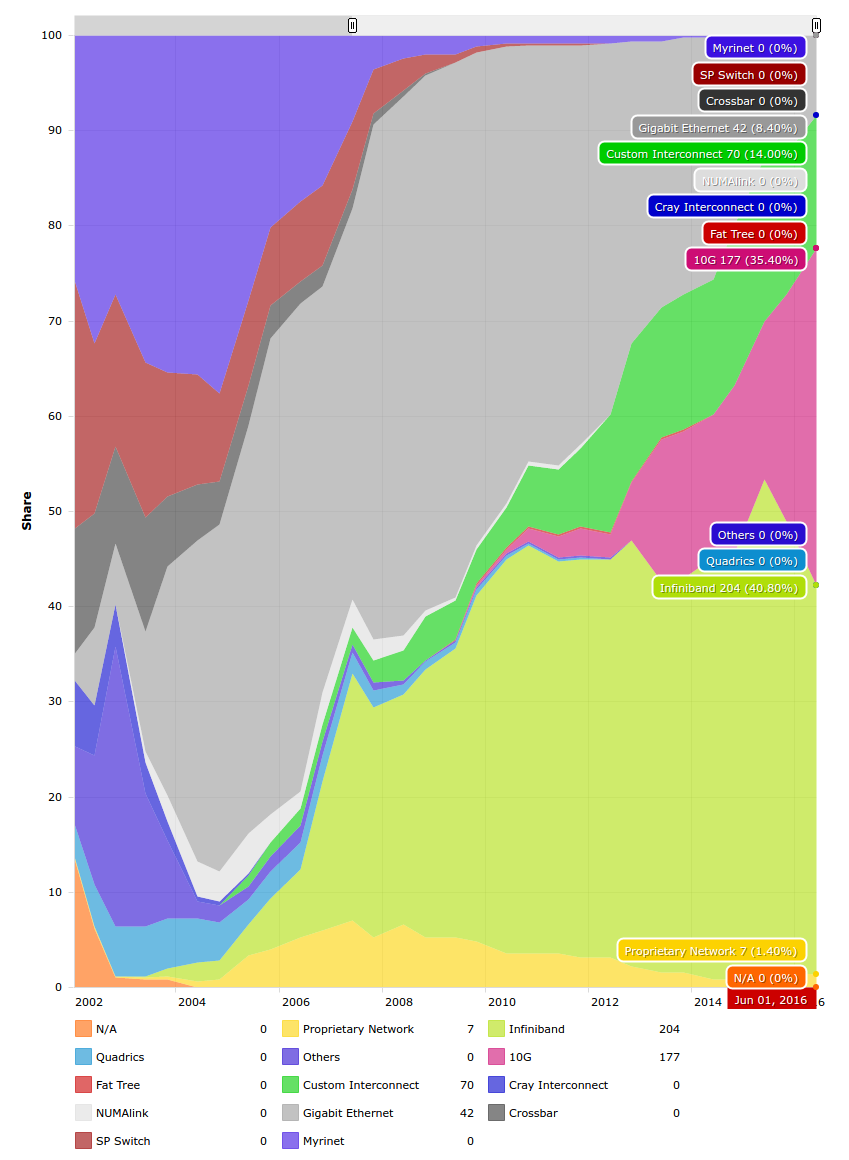
\includegraphics[width=1\linewidth]{images/top500-interconnect.png}
  \caption{Interconnect Family}
  \label{fig:sub1}
\end{subfigure}%
\begin{subfigure}{.5\textwidth}
  \centering
  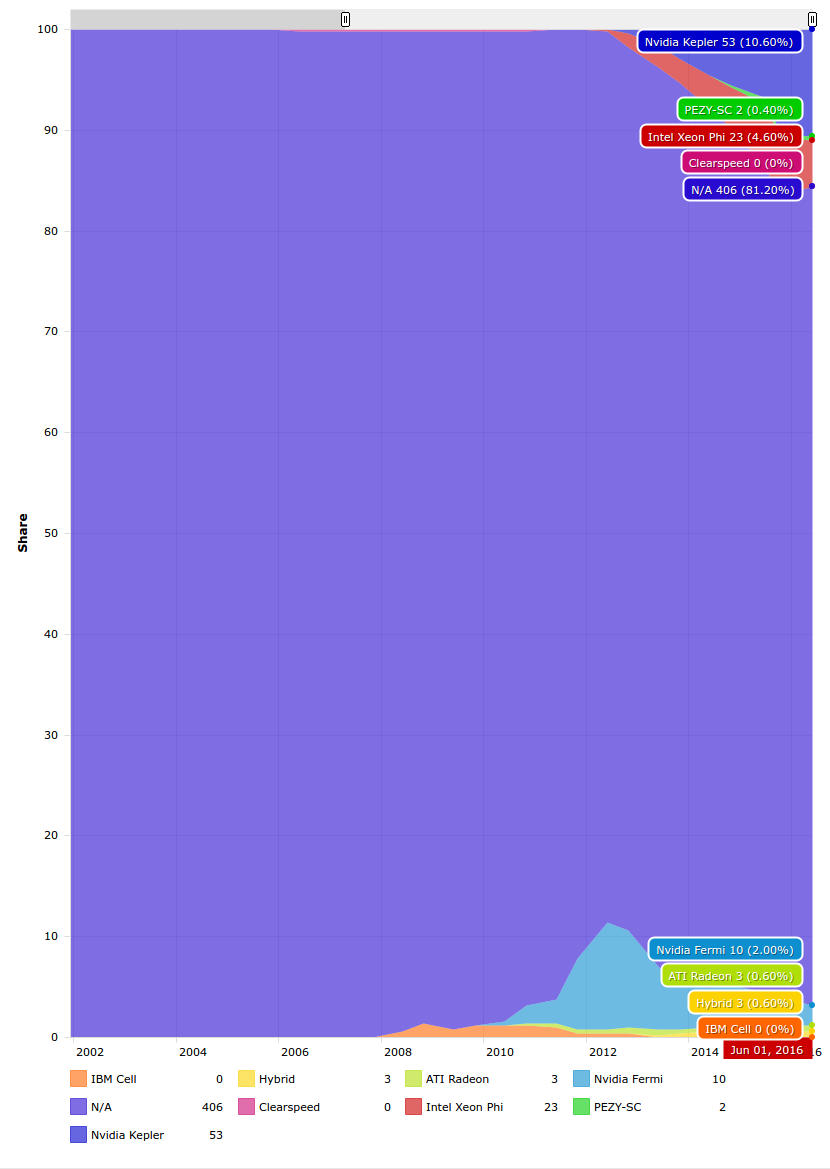
\includegraphics[width=1\linewidth]{images/top500-coprocessor.png}
  \caption{Accelerator/Coprocessor Family}
  \label{fig:sub2}
\end{subfigure}
\caption{Top 500 Development over time from 2002 to 2016 \cite{www-top500}}
\label{F:top500}
\end{figure}

\begin{comment}
\FIGURE{thb}
  {images/top500-interconnect.png}
  {1.0}
  {Interconnect Family \cite{www-top500}}
  {F:top500-interconnect}

\FIGURE{thb}
  {images/top500-coprocessor.png}
  {1.0}
  {Accelerator/Coprocessor Family \cite{www-top500}}
  {F:top500-coproc}
\end{comment}

To get an idea of some of the hardware advances over the past few years, it is useful to examine the Top 500 \cite{www-top500}, a comprehensive list of the top 500 supercomputers known and their key characteristics.  Looking at the past decade in HPC, we can see some trends emerge within hardware. Specifically looking at Interconnect and Coprocessor architectures in Figure \ref{F:top500}, we see a notable jump in the number of deployed system that are using both InfiniBand and GPUs in the past decade. Specifically, InfiniBand usage has increased to roughly 40\% of the total number of deployed systems and remained somewhat stable as an interconnect family. Concurrently, the use of accelerators has increased form only 1 in 500 systems a decade ago, to almost a 20\% of the top 500 systems that are using coprocessors. Within that factor, the majority of such accelerator-equipped systems have been using GPUs, with a concurrent increase in the Intel Xeon Phi coprocessor as well.  While these do not represent all of supercomputing nor exclusively the most high end of systems, they do represent advanced hardware that has been increasingly common in the last decade, yet relatively underutilized in comparison within cloud infrastructure. As such, much of the effort in this dissertation focuses on, but is not limited to,  these two technology families.    



%Breifly mention that it is these type of computations we woud like to support in virtualization?

\subsection{Exascale}

As the forefront of supercomputing moves beyond the latest petaflop machines in the past few years \cite{bland2012titan}, the HPC community is setting their sights on the next significant milestone: Exascale. Exascale computing refers broadly to performing roughly one exaFLOPS, or $10^{18}$ floating point operations per second. However, exascale itself is far more than just a theoretical FLOPS goal, but instead a set of new computing advancements and challenges that requires reaching computational power at such magnitude.  While FLOPs are often used as the ubiquitous yard stick for supercomputing with the LINPACK benchmark \cite{dongarra2003linpack,}, other efforts have taken hold to classify systems under a different set of parameters \cite{murphy2010graph500, dongarra2013hpcg}, with the loose understanding that these may incorporate a richer application set destined for exascale systems.  This could include for instance integer calculations at a similar scale to satisfy defence and intelligence perspectives, or graph processing at a 

With exascale, there are a number of barriers that exist with current technologies that must be overcome to reach exascale.  The exascale Computing Study \cite{bergman2008exascale} specifically lists 4 major focal areas:

\begin{enumerate}
\item Energy and Power Challenge
\begin{itemize}
\item Describes the physical difficulties in providing the amount of power needed to drive a sufficiently large exascale system. The US DOE estimates the maximum power envelope for a deployed first exascale system to be within 20-40MW. Extrapolating current technology power utilization shows an order of magnitude more energy utilization than the specificity power envelop. As such, new architectures and conversation techniques will need to be investigated. 
\end{itemize}
\item Memory and Storage Challenge 
\begin{itemize}
\item This challenge illustrates the problem that has grown in relation to the memory wall, defined by the exponential difference between processor and memory performance, as well as the storage capacity limits to support calculations at the level of performance necessary. This challenge incorporates not only main memory limitations, but also tertiary storage issues as well. 
\end{itemize}
\item Concurrency and Storage Challenge
\begin{itemize}
\item This challenge is born from the recent limit in CPU clock rates as a way to gain performance. Instead, performance must be gained through parallelism. The depth of this challenge is especially profound when we consider parallelism on the order of millions, if not billions of threads.  
\end{itemize}
\item Resiliency Challenge
\begin{itemize}
\item The resiliency challenge defines the necessity of computation to recover and continue in the event of a fault or fluctuation. As parallelism  and the number of individualized components substantially increases in a path towards exascale, the mean time to failure of any given component also increases.  
\end{itemize}
\end{enumerate}


While current exascale efforts are as wide as they are varying, not only with concepts, architectures, and runtime systems, but also with deployment plans and expectations between future deployments. Of particular interest in current exascale research is in Operating System and runtime (OS/R) developments to support new extreme-scale applications in an efficient manner. Two examples of novel OS approaches are the Hobbes project \cite{brightwell2013hobbes} and the ARGO Exascale Operating System \cite{perarnau2015argo}. These OS efforts, along with novel programming models for exascale such as ParalleX \cite{sterling2014} look to fundamentally change the relationship between HPC hardware architectures and the libraries and  applications to be leveraged on such future exascale deployments.   

 It is possible that virtualization itself may have an impact in OS and runtime services in exascale\cite{brightwell2013hobbes}. While some of the work herein may be tangentially of utility to such efforts, the immediate goal of this dissertation is not to investigate the applicability of virtualization for exascale systems, but rather to enable the diversification of HPC towards cloud infrastructure.


